%!TEX root = ../template.tex
%%%%%%%%%%%%%%%%%%%%%%%%%%%%%%%%%%%%%%%%%%%%%%%%%%%%%%%%%%%%%%%%%%%
%% chapter1.tex
%% NOVA thesis document file
%%
%% Chapter with introduction
%%%%%%%%%%%%%%%%%%%%%%%%%%%%%%%%%%%%%%%%%%%%%%%%%%%%%%%%%%%%%%%%%%%

\typeout{NT FILE chapter1.tex}%

\chapter{Introduction}
\label{cha:introduction}

\prependtographicspath{{Chapters/Figures/Covers/}}


\section{Biosignals and Challenges of a Data-Driven Society} 
\label{sub:motivation1}

%In recent years, the continuous increase in accessible wearable technology has contributed to a significant amount of data available.

It has never been easier to gather information about any aspect of our life, work, health, industry, education, and society in general. The continuous collection of data through the usage of mobile phones, smartwatches, hearables, wristbands, and other non-invasive wearable sensors leads to a large and valuable volume of information gathered in all possible scenarios. As reported in \textit{Tankovska et al.}, the use of wearable devices has more than doubled in the interval between 2016 and 2019, reaching 722 million worldwide ~\cite{tankovska_23_2020}. This data often comes in the form of time series, which is one of the most common data types in nature \cite{puttinghuman}.

A time series data type with special interest is a \textit{biosignal}. These are time series generated by the \textit{human body}, such as the \textit{heart} (\gls{ecg} - 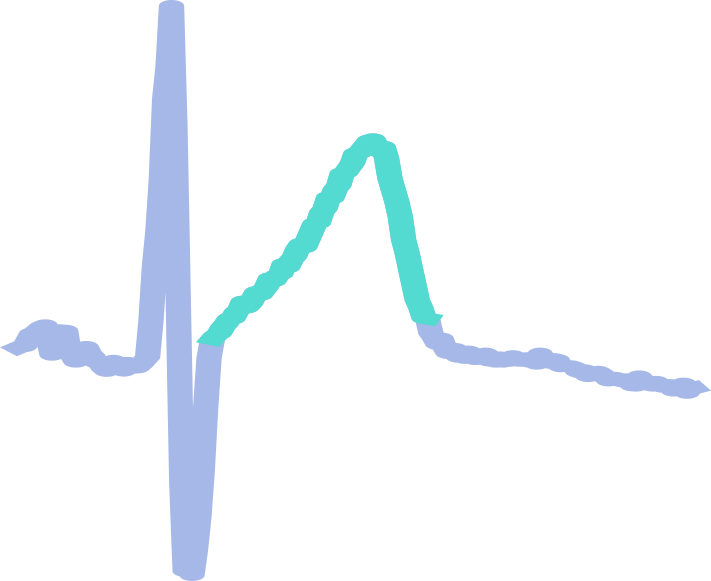
\includegraphics[height=3.5ex, valign=m]{large_peak_ecg.png}), \textit{muscles} (\gls{emg} - 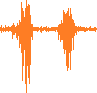
\includegraphics[height=3.5ex, valign=m]{emg_thumbnail.pdf}), \textit{brain} (\gls{eeg} - 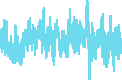
\includegraphics[height=3.5ex, valign=m]{eeg.pdf}) or even movements (\gls{imu} - 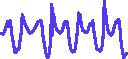
\includegraphics[height=3.5ex, valign=m]{acc_thumbnail.pdf}). The usage of such signals has emerged as Biosignal-based technology has been increasingly available in our daily lives, being widely applied in biometrics \cite{david_thesis}, human activity recognition \cite{cpd_har_1, cpd_har_2, review_1}, sports sciences \cite{li20gait, liu22activityduration, mendes2016sensor, ji2018real, howard2016survey, mcnab2011iphone, howard2016wireless, yuji2005mems, espinosa2015inertial, ohgi2002microcomputer}, healthcare \cite{cpd_medical_1, cpd_medical_2, cpd_medical_3, cpd_medical_4, dataset6, dataset7}, rehabilitation assistance \cite{rehab1, rehab2}, ergonomics \cite{antonio, sara}, and edutainment \cite{edutainment}.

Having relevant information about a specific topic can be beneficial, but the overwhelming amount of data being collected brings tremendous challenges in the ability to save, process, and analyze it, as well as retrieve interpretable and meaningful information based on which we can act upon \cite{bigdata}. Ultimately, these challenges make it difficult to have data that is well structured and labelled, considering that it is an intricate, thorough, and time-consuming process. Additionally, higher quantity of data increases the complexity of the mentioned processes. In the work of \textit{Roh et al.} it is mentioned that data scientists only rely on a small portion of the available datasets as it is too expensive to label all the data available \cite{roh2019survey}. This is just an example of how much data can have limited use or even go unused. This is particularly problematic when developing machine learning applications, as data should be correctly pre-processed and labelled for supervised approaches so it does not include noise, artifacts or mislabeled segments of the signal \cite{roh2019survey}. 

Computational methods are necessary to reduce time-consuming data-driven analysis, but the first layer of knowledge comes from the human mind and not from machines. Taking this into account, interactive data analysis is a great challenge as there is a lack of integrated interactive systems, tools and methods for fast, useful, and meaningful information retrieval from time series data \cite{intuition1, intuition2, holzinger, machado2015}. In order to do more with the data we have, tools should be available to support and help analysts to accelerate the process of information retrieval from time series. We believe that having more informative, expressive, and intuitive methods for the analysis of such data can help researchers that are familiar with time series data mining, such as data scientists, in accelerating their analysis tasks and streamline their analysis tasks. In addition, we also believe that such methods could help democratize these tasks to researchers that are not as experienced in this domain, but could benefit from it in their research activities \cite{democratize}.

In this thesis, we explore two main domains of methods for information retrieval in time series, which will be referred to as (1) \textit{unveiling the grammar of time series} and (2) \textit{a language for time series data mining}. In the first domain, we propose a practical and manageable way to automatically segment single channel or multimodal time series. The proposed approach also brings a lucid visual support in interpreting the time series and helps \textit{unveiling} its structure. The second domain focuses on using text-based approaches to search for patterns and events on time series with expressive queries, moving towards human interpretable and readable time series analysis. A novel symbolic representation of time series will be proposed and its application on query-based search and classification of time series is explored.

The presented thesis is entitled \textit{A Language for Biosignals}. It suggests that concepts and algorithms used for text in natural language processing can be applied to \textit{biosignals}. Thus, we will further explain what we believe is the \textit{linguistic nature} of time series, with a deeper focus on \textit{biosignals}.  

\section{Linguistic Nature of Biosignals} 
\label{sub:context1}

The human brain has an innate ability to identify relevant structures and patterns from the information it receives, being fundamental for decision-making \cite{cognition}. This capacity is also revealed when observing time series, and finding inherent patterns that can be associated with specific phenomenons. 
As an example, let us depict an \gls{ecg}, a typical physiological signal. The standard cyclic nature of the \gls{ecg} may be affected by several sources, such as motion artefacts, muscular contractions or even symptomatic events.
For instance, the signal piece 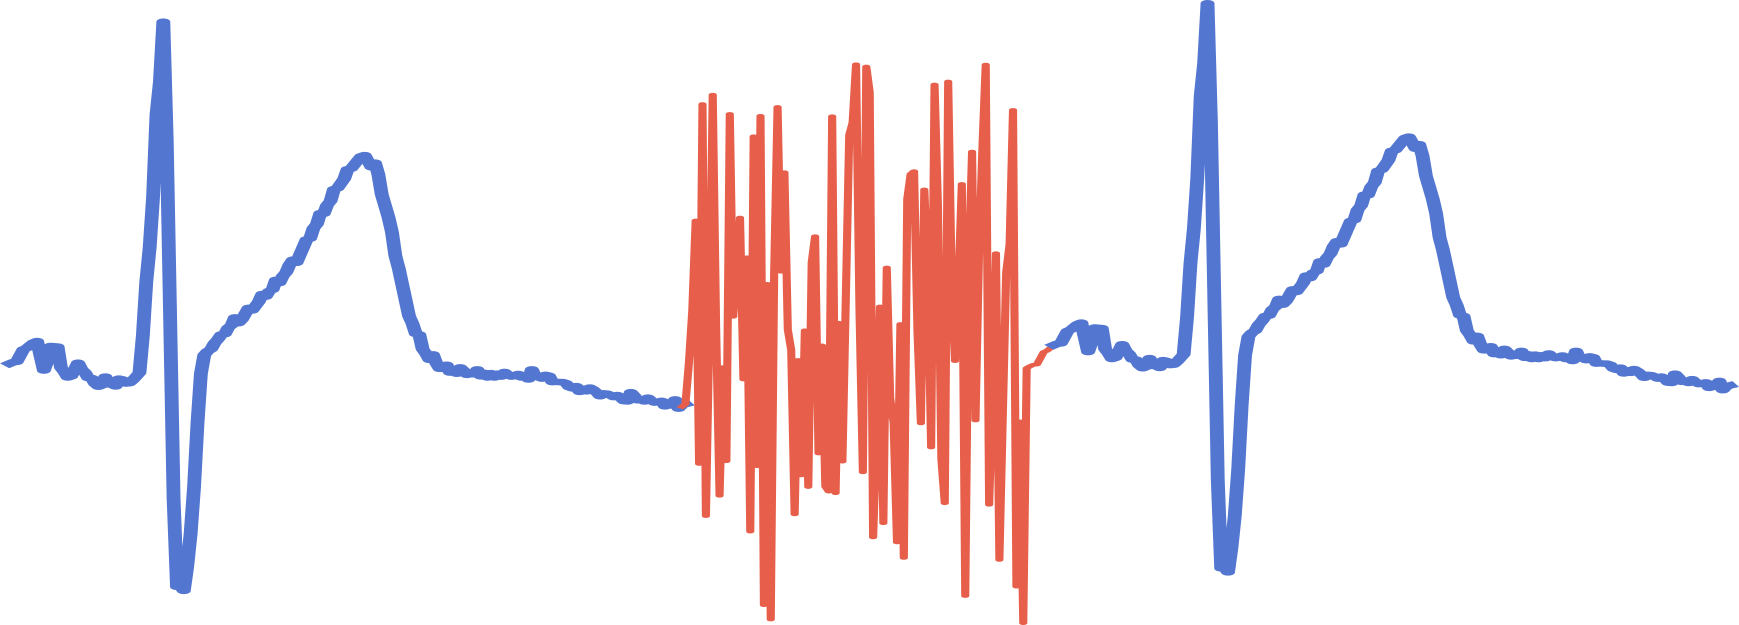
\includegraphics[height=3ex, valign=m]{ecg_noise_thumbnail.png} has two cycles of an \textcolor{myblue}{\gls{ecg}} disturbed by \textcolor{myred}{noise}. Thus we can conclude that the signal has three segments, of which two of these (the first segment and the last) have high similarity, i.e., \textit{\textcolor{myblue}{A} \textcolor{myred}{B} \textcolor{myblue}{A}}. Other changes may be related with the dynamics of the process, for instance, a subject can change and evolve his/her gait from \textcolor{myblue}{walking} to \textcolor{mygreen}{jogging} (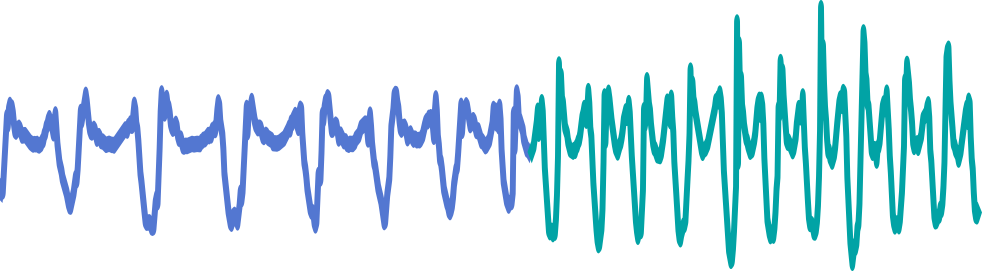
\includegraphics[height=2.5ex, valign=M]{walking_jogging.png}) — this \gls{acc} signal contains two main periodic \textit{regimes}, which could be segmented as \textcolor{myblue}{WW...W} and \textcolor{mygreen}{JJ...J}.

This visual intuition is also straightforward when an analyst is searching for specific shapes or patterns in time series. Often, the analyst resorts to describe the shape he/she is looking for. For instance, a physician may say "\textit{I am searching for the T-wave, that represents the} \texttt{wide peak}" (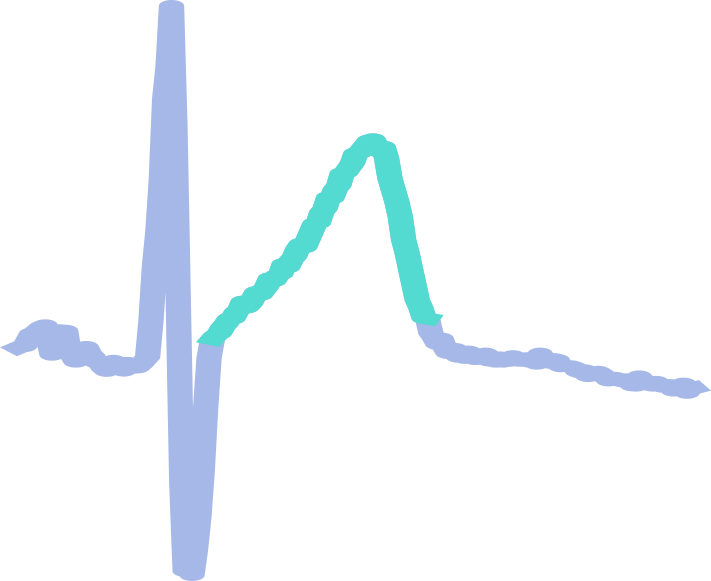
\includegraphics[height=3.5ex, valign=m]{large_peak_ecg.png}) or "\textit{I am searching for the QRS complex, that looks like a} \texttt{sharp peak followed by a sharp valley} (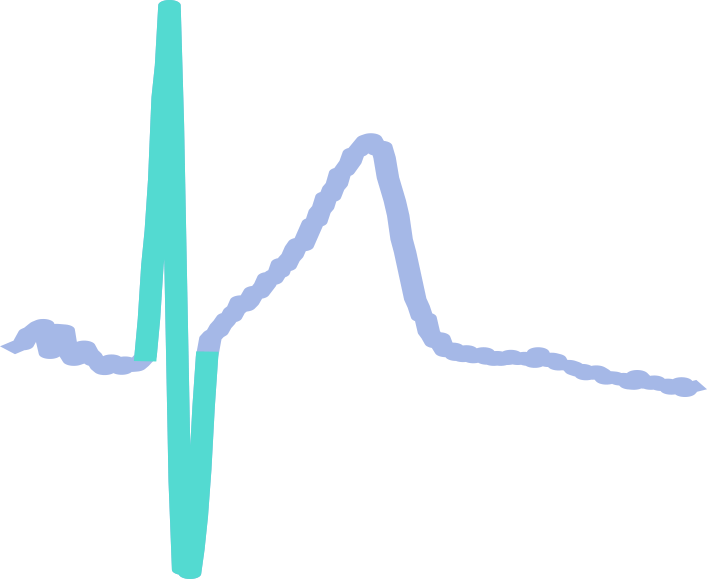
\includegraphics[height=3.5ex, valign=m]{high_peak_ecg.png})". This visual intuition also happens when analysts are trying to find differences between classes of signals. For instance, the following shapes (1) 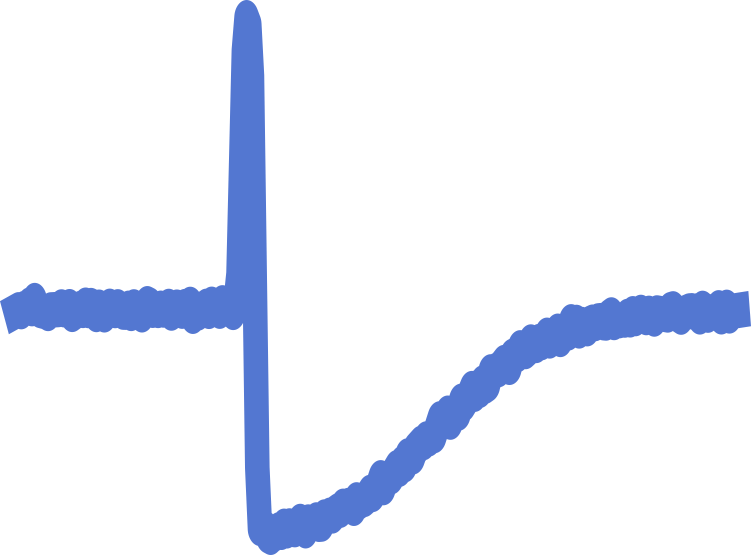
\includegraphics[height=2.5ex, width=3.5ex, valign=M]{trace1.png} and (2) 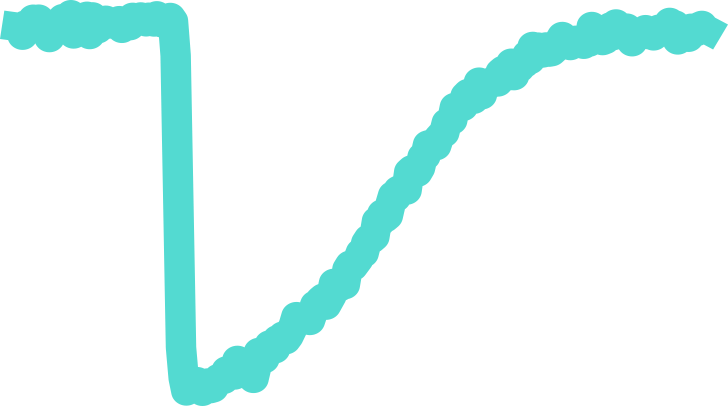
\includegraphics[height=2.5ex, width=3.5ex, valign=M]{trace_2.png} are different because "\textit{shape 1 has a} \texttt{positive peak} \textit{where shape 2 doesn't}". 

Time series are carriers of information, and the presence of changes in its \textit{regimes} or the presence of specific shapes in its segment may be associated with an occurrence in the physical world attributed to some meaning. These underlying associations that the human mind does give this notion of structure and meaning, which is a good approximation of what represents the foundation of a language: grammar and meaning~\cite{grammar}. In language, a sequence of words needs to follow a certain structure to have an interpretable meaning. In biosignals this can also be observed as the way how certain patterns are structured in the signals and allow us to extract a physiological meaning. Thus, we can pose the question: Do biosignals exhibit a certain grammar and meaning, just like language does?

\textit{Grammar} is generally defined as the set of rules that constitutes the structure of a language and is modeled by morphology and syntax \cite{grammar}. The first is the structure of words, how these are built or morphed from individual symbols based on context, while the latter consists in organizing words in sequences to form larger linguistic units, such as sentences. Just as a language has morphological and syntax rules that represent its structural information, time series can be organized by a formal structure of ordered subsegments with specific morphological characteristics, organized to build larger segments. Our first topic is related to \textit{unveiling} this structure with methods that can parse it.

In addition to a \textit{grammar}, a language also has \textit{meaning}. The \textit{meaning} regarding time series depends on the context and what occurred in the physical world that is then seen on the signal. Specific occurrences might be attributed a specific meaning by an analyst, as we have seen above with the physician example. In this work, we explore a language to \textit{translate} time series into text and use this textual information as an expressive way of searching for meaningful events and patterns. This is related to our second topic, which focuses on using language in time series data mining tasks.

Having explained how time series have a \textit{linguistic nature}, we now focus our attention to a specific domain of \textit{biosignals} and how the questions that are generally posed on time series are also valid, meaningful, and applicable to \textit{biosignals} from the occupational health context.

\section{Biosignals: Context and Relevance in Occupational Health} 
\label{sub:context2}

This thesis was developed in partnership with the \textit{Ergonomics} team from \textit{Volkswagen Autoeuropa}, with a focus on the analysis of \textit{biosignals} from workers to retrieve meaningful information about their occupational risk status and prevent \gls{wmsd}. \gls{wmsd}s prevail as the most common occupational diseases in the European Union and have a global impact on the well-being of individuals and their quality of life in a range of working sectors \cite{Irastorza2010}, accounting for the second-largest cause of disability worldwide \cite{Luttmann2003}. These are especially prevalent as upper limb or neck disorder (with 42\% of all \gls{wmsd} cases reported) \cite{Seidel2019} in several industry sectors, such as textile and automotive, where production processes with pre-defined motions and actions have a repetitive nature. This type of occupational activities have a negative impact on the well being, and making workers more prone to such disorders, with tremendous consequences to both workers and companies, namely absenteeism, early retirement, and loss of productivity \cite{Trabalhadores, Varandas19}. 

Several strategies have been implemented to identify, regulate and prevent occupational risks in manufacturing industries, such as (1) the inclusion of job rotation schedules, which promote a variation of the exposure throughout the working day \cite{jobrotation1, jobrotation2} and (2) screening tools, for the assessment of occupational risk exposure, for example the \gls{ocra}, \gls{rula} or the \gls{eaws} \cite{ocra, rula, eaws}. Nevertheless, these strategies are not optimal because they (1) are not automated, relying on observational methods and dedicated personnel to inspect video records; (2) are not objective measures; (3) do not take into account differences among the worker's population, such as anthropometric parameters, age and experience variability; and (4) present single scores, being insufficient to explain the factors that contributed to this risk. With the advent of Industry 4.0, more companies are using modern strategies that follow digital solutions to provide direct and objective quantitative measures \cite{romero}. An example of these strategies is the usage of \textit{biosignals}, with wearable inertial devices for physiological, motion, and posture tracking of workers.

From \gls{imu}, time series can be collected and relevant variables and parameters can be directly measured, such as the position and velocity of each body segment, postural angles between joints, and gait parameters, making these important for ergonomics studies \cite{Caputo2019, Hang19}. There are some limitations to using \gls{imu}, mostly related to the long-term bias (sensor drifting) arising from long acquisitions and the empirical process to fine-tune sensor fusion techniques. Other systems can be used for motion capture, such as camera-based methods, but these rely on a fixed setup of cameras, which is unfeasible in real industrial scenarios \cite{sara}. In addition to motion sensors, the inclusion of physiological sensors, such as \gls{ecg}, \gls{emg} and even \gls{fnirs} can give reliable evidence of other occupational health variables, namely cardiovascular load, muscular activation, cognitive effort and fatigue \cite{silva_rip, cardiovascular_load, rythm_cyclic_work, rui_varandas}.

The usage of biosignals in this context can play an important role in supporting the decision of ergonomists and other professionals in the industry. In order to develop systems that can use physiological, motion, and postural data for direct risk assessment and reporting, several challenges have to be answered. For instance, considering the periodic nature of most manufacturing tasks, risk factors are calculated by working cycle. Therefore, methods should be developed to identify working cycles. In addition, real occupational scenarios might have interruptions or changes in the working behaviour, due to abrupt production stoppage, shift breaks, or even because the worker shifted to another workspace that has a different movement pattern. 

Other questions brought up by ergonomists, such as \textit{can we find a pattern that has a sharp rise in the acceleration of the arm motion?} or \textit{when the worker is using a hand tool to rotate a screw, can we see a periodic pattern on the acceleration pattern from the hand?}, which represent specific patterns with a descriptive shape that can be seen on the signals and are specific of a task, need to be explored qualitatively and quantitatively. These events can be relevant to studying their precise impact on the worker's occupational exposure. Having ways to detect these patterns is of great relevance as well. In this study, we will show how the proposed solutions can have an impact on these problems, and how they contribute to providing relevant visual feedback for information retrieval and make the search for specific patterns more intuitive and expressive, even profiting from the expressiveness of the text written on the questions above.

%This would also help counteract the lack of usability of data by moving towards a \textit{democratized} usage of time series by non-experienced scientists \cite{democratize}.

\section{Research Paths}

The central objective of this work is the development of novel tools for biosignals information retrieval. Overall, the work in this thesis contributed to all layers related to \textit{biosignals}, from the moment data is acquired (\textit{sensing}), to when it is processed for information retrieval (\textit{analysis}), and how this information is used to act upon (\textit{decision-making}). These three topics were the starting point of this work. It eventually branched into several research paths, specially for the \textit{analysis} layer.
A detailed description of each of the researched layers is provided further:

\begin{enumerate}

\item \textbf{Sensing} - Explore in depth the available technology to measure motion and postural variables in occupational scenarios for risk assessment. This will take into account which variables are associated with a risk, based on ergonomic standards. These measures are returned as \textit{biosignals}, which are processed in the topic \textit{analysis};

\item \textbf{Analysis} - In this topic, two main research paths are explored: 
	\begin{enumerate}
		\item \textbf{\textit{Unveiling the Grammar of Time Series} -} Research how to perform structural information retrieval in \textit{biosignals} with a special interest in the segmentation based on \textit{novelty} and \textit{periodic} search, with applications to \textit{summarization}, and how the resulting segments are related to each other, based on their \textit{similarity}. For this, we will introduce the \textbf{\gls{ssm}}, a feature-based transformation of the signal from similarity-based measures that makes a meaningful visual representation, from which the segmentation points can be extracted and the relationship between segments can be made. 
		\item \textbf{\textit{A Language for Time Series Data Mining} - } Explore a symbolic representation of \textit{biosignals} and a word feature-based representation of \textit{biosignals}, studying how these can be used for more expressive and intuitive pattern search with the help of regular expressions, natural language and operators. In this research branch, we will introduce \gls{ssts} and \gls{quots}. 
		
From the textual representation of time series, we also explored how to make a higher level distance measure, following standard text mining methods. The resulting outputs of these methods can ultimately be used to have more hints of why a signal is different from another. This path will introduce \gls{hearts}.

	\end{enumerate}

\item \textbf{Decision-Making -} Discuss how the developed methods can contribute to more aware and informed decisions. Considering the outputs of the methods developed in research path \textbf{2.a - Analysis - Unveiling the Grammar of Time Series}, how can the analyst gain intuition over the structure of the data associating it with what happened in the physical world? With regards to research path \textbf{2.b - Analysis - A Language for Time Series Data Mining}, how expressive is the process of searching for specific events and patterns with the proposed linguistic-based search methods?

\end{enumerate}

\section{Thesis Structure}
\label{sec:structure}

\begin{figure}[h]
\centering
\includegraphics[width=\linewidth]{intro_structure.pdf}
\caption{General topics on this thesis and structure of the document. It highlights the 3 layers of involvement related to time series: Sensing, Analysis, and Decision-Making, focusing on the Analysis layer, which includes two major topics subdivided into 4 sections each.}
\label{fig:intro}
\end{figure}

This thesis provides a detailed description and explanation of the research work developed during the Ph.D. program. It is organized into seven main Chapters and two Appendixes, each emphasizing on the scientific contributions developed throughout this thesis. Figure \ref{fig:intro} illustrates of the structure of this work with each Chapter's topics and content. \textbf{Chapter 1 - Introduction -} has introduced the main motivations, goals, and context for the development of the proposed methods. \textbf{Chapter 2 - Time Series Fundamentals -} explains the fundamental definitions and knowledge needed to have a clear picture of what is developed in this work. \textbf{Chapter 3 - State-of-the-art -} depicts the literature review of related work, namely in the topics of segmentation, summarization, pattern/event search, and classification, with a focus in \textit{biosignals}. \textbf{Chapter 4 - Unveiling the grammar of time series -} explains the algorithm developed for time series structural information retrieval and provides examples of its usage for novelty segmentation, periodic segmentation, similarity profiles, query-based search and summarization. \textbf{Chapter 5 - A language for time series data mining -} covers the usage of language for time series data mining, more specifically introducing a novel symbolic approximation and how it can be used for pattern search and classification. In addition, it also explains how to use natural language with a word-feature-based representation of time series. \textbf{Chapter 6 - Experimental Analysis, Validation and Discussion -} shows the application of the previous methods to a set of examples, and presents major results that validate the performance of the proposed methods. In addition, this chapter also provides a general discussion of the results and how the proposed methods can be used for the benefit of the analyst. \textbf{Chapter 7 - Conclusion and Future Work -} gives an overall remark on the outcomes of this thesis and a reflection on the contributions that the developed methods have in making time series preparation and data mining more expressive, quicker, and more practical for an ever-increasing number of data available. It also gives a clear idea of which are the future paths for this work in terms of novel applications and performance improvement.

Two Appendixes are also part of this work and give additional information on the datasets used, algorithms and results. \textbf{Appendix 1 - Data description and management -} describes the data we used, explaining its source for both private data and publicly available data, for which purposes it was used and how it was used in this work. \textbf{Appendix 2 - Detailed Results for Information Retrieval and Classification -} gives more non-fundamental information about the methods developed, and detailed results, namely of the algorithm's performance in each record of the datasets, and hyperparameters used.